\documentclass[../main.tex]{subfiles}

\begin{document}
\part{Part Six}



\begin{center}\begin{Large}\textbf{Ordinary Differential Equations}\end{Large}\end{center}



\Large{6.1 \; OVERVIEW}\\
\hrule
\vspace{0,5 cm}
The fundamental laws of physics, mechanics, electricity, and thermodynamics are usually
based on empirical observations that explain variations in physical properties and states of
systems. Rather than describing the state of physical systems directly, the laws are usually
couched in terms of spatial and temporal changes. These laws define mechanisms of
change. When combined with continuity laws for energy, mass, or momentum, differential
equations result. Subsequent integration of these differential equations results in mathematical functions that describe the spatial and temporal state of a system in terms of energy,
mass, or velocity variations. As in Fig. PT6.1, the integration can be implemented analytically with calculus or numerically with the computer. The free-falling bungee jumper problem introduced in Chap. 1 is an example of the derivation of a differential equation from a fundamental law. Recall that Newton's second law
was used to develop an ODE describing
the rate of change of velocity of a falling
bungee jumper:
\begin{equation}
\tag{PT6.1}
\dfrac{dv}{dt} = g - \dfrac{c_{d}}{m} v^{2}
\end{equation}\\
where g is the gravitational constant, m is
the mass, and cd is a drag coefficient.
Such equations, which are composed of
an unknown function and its derivatives,
are called $differential equations$. They
are sometimes referred to as $rate equations$ because they express the rate of
change of a variable as a function of variables and parameters.

In Eq. (PT6.1), the quantity being
differentiated v is called the $dependent
variable$. The quantity with respect to
which $v$ is differentiated $t$ is called the
$independent variable$. When the function
\pagebreak
\begin{figure}[hbt!]
	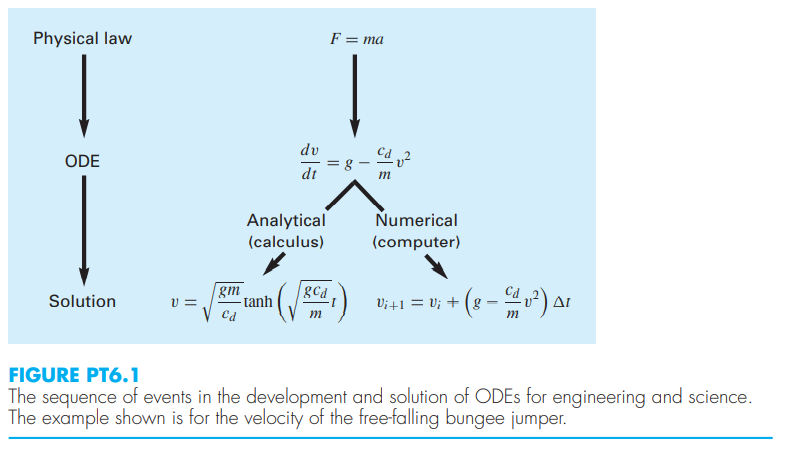
\includegraphics[width=0.95\textwidth]{PT6.1}
	\label{PT6.1}
\end{figure}\\
involves one independent variable, the equation is called an $ordinary differential equation$ (or ODE). This is in contrast to a $partial differential equation$ (or PDE) that involves two
or more independent variables.

Differential equations are also classified as to their $order$. For example, Eq. (PT6.1) is
called a $first-order equation$ because the highest derivative is a first derivative. A $secondorder equation$ would include a second derivative. For example, the equation describing the
position x of an unforced mass-spring system with damping is the second-order equation:
\begin{equation}
\tag{PT6.2}
m\dfrac{d^{2}x}{dt^{2}} + c\dfrac{dx}{dt} + kx = 0
\end{equation}\\
where $m$ is mass, $c$ is a damping coefficient, and $k$ is a spring constant. Similarly, an nthorder equation would include an $n$th derivative.
Higher-order differential equations can be reduced to a system of first-order equations.
This is accomplished by defining the first derivative of the dependent variable as a new
variable. For Eq. (PT6.2), this is done by creating a new variable v as the first derivative of
displacement
\begin{equation}
\tag{PT6.3}
v=\dfrac{dx}{dt}
\end{equation}\\
where $v$ is velocity. This equation can itself be differentiated to yield
\begin{equation}
\tag{PT6.4}
\dfrac{dv}{dt} = \dfrac{d^{2}x}{dt^{2}}
\end{equation}\\
Equations (PT6.3) and (PT6.4) can be substituted into Eq. (PT6.2) to convert it into a firstorder equation:\\
\begin{equation}
\tag{PT6.5}
m\dfrac{dv}{dt} + cv + kx = 0
\end{equation}\\
As a final step, we can express Eqs. (PT6.3) and (PT6.5) as rate equations:\\
\begin{equation}
\tag{PT6.6}
\dfrac{dx}{dt} = v
\end{equation}\\
\begin{equation}
\tag{PT6.7}
\dfrac{dv}{dt} = -\dfrac{c}{m}v - \dfrac{k}{m} x
\end{equation}\\
Thus, Eqs. (PT6.6) and (PT6.7) are a pair of first-order equations that are equivalent
to the original second-order equation (Eq. PT6.2). Because other nth-order differential
equations can be similarly reduced, this part of our book focuses on the solution of firstorder equations.

A solution of an ordinary differential equation is a specific function of the independent
variable and parameters that satisfies the original differential equation. To illustrate this
concept, let us start with a simple fourth-order polynomial,\\
\begin{equation}
\tag{PT6.8}
y=-0.5x^4 + 4x^3 - 10x^2 + 8.5x + 1
\end{equation}\\
Now, if we differentiate Eq. (PT6.8), we obtain an ODE:
\begin{equation}
\tag{PT6.9}
\dfrac{dy}{dx} = -2x^3 + 12x^2 - 20x + 8.5
\end{equation}\\
This equation also describes the behavior of the polynomial, but in a manner different from
Eq. (PT6.8). Rather than explicitly representing the values of y for each value of x,
Eq. (PT6.9) gives the rate of change of $y$ with respect to $x$ (i.e., the slope) at every value of
$x$. Figure PT6.2 shows both the function and the derivative plotted versus x. Notice how the
zero values of the derivatives correspond to the point at which the original function is
flat—that is, where it has a zero slope. Also, the maximum absolute values of the derivatives are at the ends of the interval where the slopes of the function are greatest.
Although, as just demonstrated, we can determine a differential equation given the
original function, the object here is to determine the original function given the differential
equation. The original function then represents the solution. 
Without computers, ODEs are usually solved analytically with calculus. For example,
Eq. (PT6.9) could be multiplied by $dx$ and integrated to yield\\
\begin{equation}
\tag{PT6.10}
y= \int(-2x^3 + 12x^2 - 20x + 8.5)dx
\end{equation}\\
The right-hand side of this equation is called an $indefinite integral$ because the limits of integration are unspecified. This is in contrast to the $definite integrals$ discussed previously
in Part Five [compare Eq. (PT6.10) with Eq. (19.5)].

An analytical solution for Eq. (PT6.10) is obtained if the indefinite integral can be evaluated exactly in equation form. For this simple case, it is possible to do this with the result:\\
\begin{equation}
\tag{PT6.11}
y=-0.5x^4 + 4x^3 - 10x^2 + 8.5x + C
\end{equation}\\
which is identical to the original function with one notable exception. In the course of differentiating and then integrating, we lost the constant value of 1 in the original equation
and gained the value C. This C is called a constant of integration. The fact that such an
arbitrary constant appears indicates that the solution is not unique. In fact, it is but one of\\
\pagebreak
\begin{figure}[hbt!]
	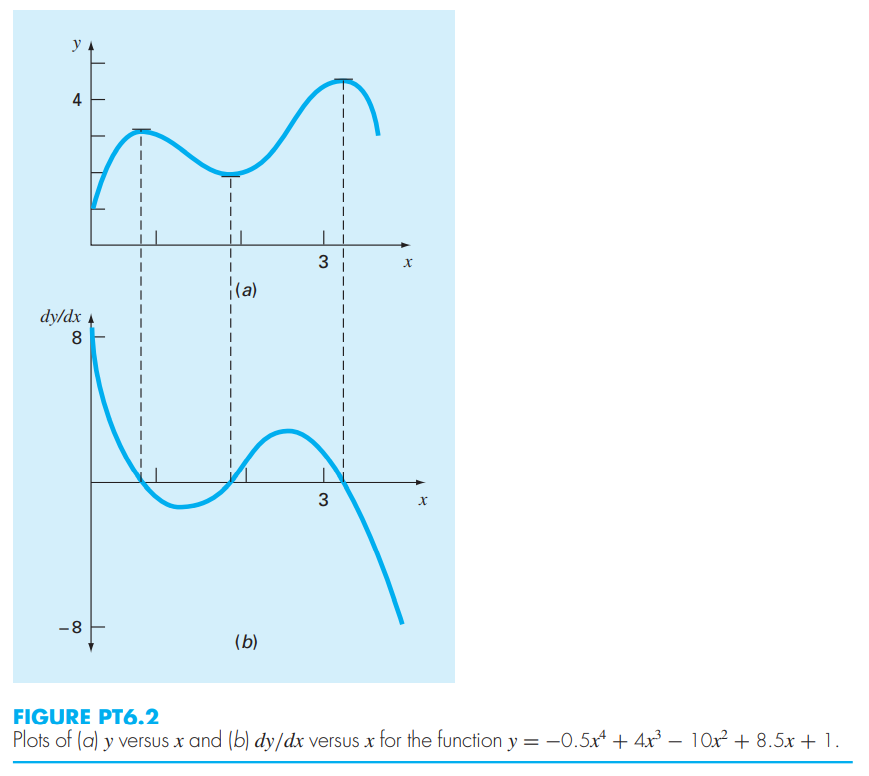
\includegraphics[width=0.95\textwidth]{PT6.2}
	\label{PT6.2}
\end{figure}\\
an infinite number of possible functions (corresponding to an infinite number of possible
values of C) that satisfy the differential equation. For example, Fig. PT6.3 shows six possible functions that satisfy Eq. (PT6.11).

Therefore, to specify the solution completely, a differential equation is usually accompanied by auxiliary conditions. For first-order ODEs, a type of auxiliary condition called
an initial value is required to determine the constant and obtain a unique solution. For
example, the original differential equation could be accompanied by the initial condition
that at x = 0, y = 1. These values could be substituted into Eq. (PT6.11) to determine
C = 1. Therefore, the unique solution that satisfies both the differential equation and the
specified initial condition is

$y=-0.5x^4 + 4x^3 - 10x^2 + 8.5 + 1$\\
Thus, we have “pinned down” Eq. (PT6.11) by forcing it to pass through the initial condition, and in so doing, we have developed a unique solution to the ODE and have come full
circle to the original function [Eq. (PT6.8)].\\
\begin{figure}[hbt!]
	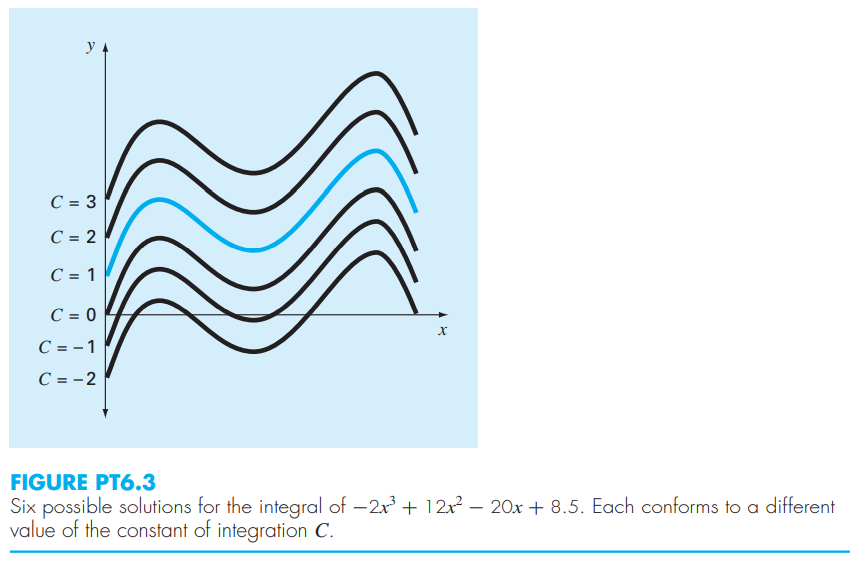
\includegraphics[width=0.95\textwidth]{PT6.3}
	\label{PT6.3}
\end{figure}\\
initial condition was reflective of the physical fact that at time zero the vertical velocity
was zero. If the bungee jumper had already been in vertical motion at time zero, the solution would have been modified to account for this initial velocity.

When dealing with an $n$th-order differential equation, $n$ conditions are required to obtain a unique solution. If all conditions are specified at the same value of the independent
variable (e.g., at $x$ or $t = 0$), then the problem is called an $initial-value problem$. This is in
contrast to $boundary-value problems$ where specification of conditions occurs at different
values of the independent variable. Chapters 22 and 23 will focus on initial-value problems. Boundary-value problems are covered in Chap. 24.\\
\vspace{0,2 cm}\\
\Large{6.1 \; OVERVIEW}\\
\hrule
\vspace{0,5 cm}
$Chapter 22$ is devoted to one-step methods for solving initial-value ODEs. As the name
suggests, $one-step methods$ compute a future prediction $y_{i+1}$, based only on information at
a single point $y_{i}$ and no other previous information. This is in contrast to $multistep approaches$ that use information from several previous points as the basis for extrapolating to
a new value.

With all but a minor exception, the one-step methods presented in Chap. 22 belong to
what are called $Runge-Kutta techniques$. Although the chapter might have been organized
around this theoretical notion, we have opted for a more graphical, intuitive approach to introduce the methods. Thus, we begin the chapter with $Euler's method$, which has a very
straightforward graphical interpretation. In addition, because we have already introduced
Euler's method in Chap. 1, our emphasis here is on quantifying its truncation error and describing its stability. 

Next, we use visually oriented arguments to develop two improved versions of Euler's
method—the $Heun$ and the $midpoint$ techniques. After this introduction, we formally develop the concept of Runge-Kutta (or RK) approaches and demonstrate how the foregoing
techniques are actually first- and second-order RK methods. This is followed by a discussion of the higher-order RK formulations that are frequently used for engineering and
scientific problem solving. In addition, we cover the application of one-step methods to
$systems of$ ODEs. Note that all the applications in Chap. 22 are limited to cases with a fixed
step size.

In Chap. 23, we cover more advanced approaches for solving initial-value problems.
First, we describe $adaptive$ RK $methods$ that automatically adjust the step size in response
to the truncation error of the computation. These methods are especially pertinent as they
are employed by MATLAB to solve ODEs.

Next, we discuss $multistep methods$. As mentioned above, these algorithms retain information of previous steps to more effectively capture the trajectory of the solution. They
also yield the truncation error estimates that can be used to implement step-size control. We
describe a simple method—the $non-self-starting Heun$ method—to introduce the essential
features of the multistep approaches.

Finally, the chapter ends with a description of $stiff$ ODEs. These are both individual
and systems of ODEs that have both fast and slow components to their solution. As a consequence, they require special solution approaches. We introduce the idea of an $implicit
solution$ technique as one commonly used remedy. We also describe MATLAB's built-in
functions for solving stiff ODEs.

In $Chap. 24$, we focus on two approaches for obtaining solutions to $boundary-value
problems$: the $shooting$ and $finite-difference methods$. Aside from demonstrating how these
techniques are implemented, we illustrate how they handle $derivative boundary conditions$
and $nonlinear$ ODEs.















	
	
	
	


\end{document}